\section{Comparison to State-of-the-art}\label{sec:vs_clsmith}

In this section we compare DeepSmith to CLSmith~\cite{Lidbury2015a}, the state-of-the-art in OpenCL compiler testing.

\subsection{Experimental Setup}

We ran each program generator using its default configuration for 48 hours on each of the 10 testbeds of Table~\ref{tab:platforms}. We ran the tests twice, first with optimizations disabled ($-$), then with optimizations enabled ($+$). Total runtime for a test-case consists of the generation time, and the time to execute the test-case. For DeepSmith, the time to generate test-harness is included.


\subsection{Results Overview}

\begin{table*}
  \scriptsize %
  \centering %
    \begin{tabular}{lll | rrrrrrr | rrrrrrr }
  \toprule
  & & & \multicolumn{7}{c|}{\textbf{CLSmith}} & \multicolumn{7}{c}{\textbf{CLgen}} \\
  \textbf{\#.} & \textbf{Device} & $\pm$ &
  \textbf{bf} & \textbf{bc} & \textbf{bto} & \textbf{c} & \textbf{to} & \cmark & \textbf{total} &
  \textbf{bf} & \textbf{bc} & \textbf{bto} & \textbf{c} & \textbf{to} & \cmark & \textbf{total} \\
  \midrule
  \multirow{ 2}{*}{1} & \multirow{ 2}{*}{GeForce GTX 1080} & $-$ & 375 & 0 & 3 & 68 & 423 & 4267 & 5136       & 20063 & 13 & 0 & 910 & 42 & 8116 & 29144 \\& & $+$ & 404 & 0 & 0 & 44 & 517 & 4586 & 5551 & 22958 & 13 & 0 & 789 & 36 & 6720 & 30516 \\
\hline
\multirow{ 2}{*}{2} & \multirow{ 2}{*}{GeForce GTX 780} & $-$ & 488 & 12 & 3 & 16 & 620 & 5567 & 6706       & 10593 & 18 & 141 & 1059 & 124 & 10116 & 22051* \\& & $+$ & 504 & 0 & 0 & 32 & 658 & 5689 & 6883 & 10679 & 18 & 131 & 1091 & 112 & 10020 & 22051* \\
\hline
\multirow{ 2}{*}{3} & \multirow{ 2}{*}{Intel HD Haswell GT2} & $-$ & 166 & 938 & 894 & 0 & 0 & 269 & 2267       & 33838 & 215 & 60 & 2474 & 0 & 22049 & 58636 \\& & $+$ & 165 & 939 & 893 & 0 & 0 & 265 & 2262 & 26684 & 183 & 59 & 1506 & 0 & 20283 & 48715* \\
\hline
\multirow{ 2}{*}{4} & \multirow{ 2}{*}{Intel E5-2620 v4} & $-$ & 1103 & 173 & 22 & 513 & 448 & 4858 & 7117       & 35858 & 94 & 38 & 2205 & 82 & 13327 & 51604 \\& & $+$ & 1051 & 0 & 4 & 493 & 592 & 4586 & 6726 & 34068 & 53 & 0 & 2284 & 152 & 13554 & 50111 \\
\hline
\multirow{ 2}{*}{5} & \multirow{ 2}{*}{Intel E5-2650 v2} & $-$ & 412 & 35 & 63 & 68 & 477 & 4577 & 5632       & 10290 & 364 & 110 & 1216 & 60 & 10090 & 22130* \\& & $+$ & 483 & 0 & 3 & 8 & 623 & 5531 & 6648 & 10340 & 370 & 103 & 1232 & 81 & 10004 & 22130* \\
\hline
\multirow{ 2}{*}{6} & \multirow{ 2}{*}{Intel i5-4570} & $-$ & 1178 & 184 & 18 & 12 & 523 & 5792 & 7707       & 12027 & 452 & 120 & 1262 & 55 & 11722 & 25638* \\& & $+$ & 1065 & 0 & 2 & 9 & 640 & 5125 & 6841 & 14527 & 460 & 168 & 1257 & 87 & 14026 & 30525* \\
\hline
\multirow{ 2}{*}{7} & \multirow{ 2}{*}{Intel Xeon Phi} & $-$ & 134 & 10 & 503 & 0 & 105 & 1041 & 1793       & 8606 & 47 & 21 & 686 & 115 & 5781 & 15256 \\& & $+$ & 370 & 0 & 24 & 171 & 449 & 4020 & 5034 & 8621 & 38 & 3 & 671 & 140 & 5660 & 15133 \\
\hline
\multirow{ 2}{*}{8} & \multirow{ 2}{*}{Intel E5-2620 (POCL)} & $-$ & 468 & 0 & 2 & 15 & 585 & 5351 & 6421       & 31564 & 39 & 0 & 2478 & 40 & 9834 & 43955 \\& & $+$ & 486 & 0 & 0 & 64 & 602 & 5541 & 6693 & 31209 & 40 & 0 & 2405 & 62 & 8973 & 42689 \\
\hline
\multirow{ 2}{*}{9} & \multirow{ 2}{*}{Intel E5-2620 (ComputeAorta)} & $-$ & 493 & 0 & 0 & 200 & 668 & 5722 & 7083       & 10801 & 698 & 105 & 359 & 17 & 10145 & 22125* \\& & $+$ & 409 & 0 & 0 & 5 & 569 & 4873 & 5856* & 10855 & 816 & 124 & 318 & 12 & 10000 & 22125* \\
\hline
\multirow{ 2}{*}{10} & \multirow{ 2}{*}{Oclgrind Simulator} & $-$ & 142 & 0 & 0 & 0 & 188 & 1623 & 1953       & 33246 & 2309 & 0 & 1084 & 279 & 10691 & 47609 \\& & $+$ & 140 & 0 & 0 & 0 & 190 & 1587 & 1917 & 31357 & 2182 & 0 & 1046 & 298 & 10346 & 45229 \\
  \bottomrule
\end{tabular}


  \caption{%
    Results from 48 hours of testing using CLSmith and DeepSmith. Testbed \#. as per Table~\ref{tab:platforms}. $\pm$ denotes optimizations off ($-$) vs on ($+$). The remaining columns denote build failure (\textbf{bf}), build crash (\textbf{bc}), build timeout (\textbf{bto}), runtime crash (\textbf{c}), timeout (\textbf{to}), and passed (\textbf{\cmark}) outcomes for CLSmith and DeepSmith, respectively.%
  }
  \label{tab:outcomes}
\end{table*}

Table~\ref{tab:outcomes} shows the outcomes of 48 hours of consecutive testing for each of the platforms from Table~\ref{tab:platforms}, with compiler optimizations disabled ($-$) and optimizations enabled ($+$).

An average of XX CLSmith and XX DeepSmith test-cases were evaluated on each device, with an average time per test-case of XX and XX respectively. The XX-fold increase in testing throughput achieved by DeepSmith is a result of XXX. Figure~\ref{fig:runtimes} shows the times taken to generate and execute test-cases. DeepSmith generation time is proportional to program length, benchmarked at an average 465 chars / second. For Clsmith, generation time depends on the number of rejections which are required before production of statically verified code is correct \cc{ldots}.

Optimization level generally does not affect testing throughput significantly, with the exception of testbed $7+$, in which the slow compilation of kernels containing structs greatly reduces the number of test-cases evaluated. This is a result of CLSmith's heavy reliance on structs, and is a known issue --- in XX the authors omnit testing on this testbed for this reason.

83.8\% of CLSmith test-cases produce a majority \textbf{\cmark} outcome. Proportionally, DeepSmith test-cases are less likely to produce a majority outcome at 47.9\% of the total. Neither CLSmith or DeepTune guarantee program termination with XX\% of non-\textbf{\{bf,c\}} majority outcomes reaching 60 seconds timeouts.


\subsection{Comparison of Results}

CLSmith crashed 8 of the 20 compilers, DeepSmith crashed all of them. See Section X for examples of bugs found from build crashes.

For all except testbed $3\pm$, DeepSmith exposes more compiler crashes than CLSmith. On average, DeepSmith hangs the compiler more frequently. \cc{\ldots}

The integrated GPU Conifgs.\ we tested ($3\pm$) frequently failed to compile CLSmith kernels, resulting in thousands of compiler crashes \textbf{bc} or timeouts \textbf{bc}.
% SELECT stderr,COUNT(*) FROM CLSmithResults LEFT JOIN CLSmithMetas ON CLSmithResults.id=CLSmithMetas.id WHERE testbed_id=13 AND CLSmithResults.outcome='bc' AND cumtime < 48 * 3600 GROUP BY CLSmithResults.stderr;
Of the build crashes, 68\% failed silently, and the remainder were caused by the same pointer assignment assertion for which DeepSmith generated a 4 line test-case in Figure~\ref{lst:intel-llvm-assertion}. \cc{We also generated silent build crashes, but with an average line count of XX, versus CLSmith's line count of XX.}

% 622 total bc
Testbeds $4$, $5$, $6$, and $7$ have a number CLSmith bc outcomes when optimizations are enabled. Of the non-silent crashes, the cause is the OpenCL vectorizer pass, same as Figure~\ref{lst:intel-vectorizer-segfault}.

\cc{Testbeds $4$, $6$ are the same driver on different hardware, and exhibit similar behavior}


\subsection{Differential Tests}

Table~\ref{tab:classifications} shows the results of applying voting heuristics to the results of Table~\ref{tab:outcomes}.

\begin{figure}
	\centering %
	\includegraphics[width=\columnwidth]{build/img/runtimes}%
	\caption{%
		Runtimes, excluding timeouts. On average, DeepSmith test-cases are evaluated $XX\times$ faster than CLSmith ($2.45\times$, $4.46\times$, and $66.54\times$ for generation, execution and reduction, respectively).%
%    Total speedup is 3.03x
%    CLgen generation is 2.45x faster than CLSmith
%    CLgen execution is 4.46x faster than CLSmith
%    CLgen reduction is 66.54x faster than CLSmith
	}%
	\label{fig:runtimes} %
\end{figure}


\begin{table*}
	\scriptsize %
	\centering %
	\begin{tabular}{lll | rrrrr | rrrrr }
  \toprule
  & & & \multicolumn{5}{c|}{\textbf{CLSmith}} & \multicolumn{5}{c}{\textbf{CLgen}} \\
  \textbf{\#.} & \textbf{Device} & $\pm$ &
  \textbf{w} & \textbf{bf} & \textbf{c} & \textbf{to} & \textbf{\% of total} &
  \textbf{w} & \textbf{bf} & \textbf{c} & \textbf{to} & \textbf{\% of total} \\
  \midrule
  \multirow{ 2}{*}{1} & \multirow{ 2}{*}{GeForce GTX 1080} & $-$ & 0 & 0 & 17 & 25 & 0.8\%       & 10 & 45 & 28 & 5 & 0.4\% \\& & $+$ & 5 & 0 & 63 & 15 & 1.5\% & 14 & 28 & 12 & 14 & 0.3\% \\
\hline
\multirow{ 2}{*}{2} & \multirow{ 2}{*}{GeForce GTX 780} & $-$ & 3 & 0 & 22 & 37 & 0.9\%       & 617 & 406 & 65 & 42 & 25.9\% \\& & $+$ & 0 & 0 & 10 & 37 & 0.7\% & 281 & 375 & 37 & 68 & 22.9\% \\
\hline
\multirow{ 2}{*}{3} & \multirow{ 2}{*}{Intel HD Haswell GT2} & $-$ & 0 & 0 & 0 & 0 & 0.0\%       & 108 & 473 & 20 & 0 & 1.2\% \\& & $+$ & 0 & 0 & 0 & 0 & 0.0\% & 22 & 39 & 6 & 0 & 0.2\% \\
\hline
\multirow{ 2}{*}{4} & \multirow{ 2}{*}{Intel E5-2620 v4} & $-$ & 0 & 563 & 192 & 0 & 11.2\%       & 3 & 10 & 93 & 1 & 0.3\% \\& & $+$ & 0 & 595 & 434 & 1 & 14.5\% & 1 & 7 & 110 & 3 & 0.3\% \\
\hline
\multirow{ 2}{*}{5} & \multirow{ 2}{*}{Intel E5-2650 v2} & $-$ & 0 & 0 & 0 & 0 & 0.0\%       & 2 & 65 & 131 & 1 & 23.9\% \\& & $+$ & 0 & 0 & 61 & 0 & 1.1\% & 8 & 66 & 138 & 3 & 25.1\% \\
\hline
\multirow{ 2}{*}{6} & \multirow{ 2}{*}{Intel i5-4570} & $-$ & 0 & 570 & 0 & 0 & 8.3\%       & 15 & 362 & 156 & 10 & 20.2\% \\& & $+$ & 0 & 629 & 0 & 0 & 8.2\% & 6 & 167 & 170 & 10 & 31.6\% \\
\hline
\multirow{ 2}{*}{7} & \multirow{ 2}{*}{Intel Xeon Phi} & $-$ & 6 & 0 & 131 & 5 & 2.8\%       & 19 & 30 & 0 & 73 & 0.9\% \\& & $+$ & 1 & 0 & 0 & 4 & 0.3\% & 12 & 32 & 0 & 65 & 0.8\% \\
\hline
\multirow{ 2}{*}{8} & \multirow{ 2}{*}{POCL (Intel E5-2620)} & $-$ & 0 & 0 & 56 & 2 & 0.9\%       & 2 & 6 & 850 & 7 & 2.8\% \\& & $+$ & 0 & 0 & 8 & 18 & 0.4\% & 1 & 7 & 930 & 1 & 2.9\% \\
\hline
\multirow{ 2}{*}{9} & \multirow{ 2}{*}{ComputeAorta (Intel E5-2620)} & $-$ & 0 & 0 & 0 & 11 & 0.2\%       & 15 & 620 & 85 & 0 & 38.8\% \\& & $+$ & 9 & 0 & 177 & 35 & 3.1\% & 19 & 563 & 49 & 6 & 39.4\% \\
\hline
\multirow{ 2}{*}{10} & \multirow{ 2}{*}{Oclgrind Simulator} & $-$ & 0 & 0 & 0 & 8 & 0.4\%       & 6 & 3 & 13 & 80 & 0.3\% \\& & $+$ & 0 & 0 & 0 & 14 & 0.7\% & 7 & 2 & 9 & 50 & 0.2\% \\
  \bottomrule
\end{tabular}


	\caption{Using voting heuristics to expose anomalous results from 48 hours of testing using CLSmith and DeepSmith. Columns denote anomalous-output (ao), anomalous build failure (\textbf{abf}), anomalous runtime crash (\textbf{ac}), and anomalous timeout (\textbf{ato}) classifications for CLSmith and DeepSmith, respectively.}
	\label{tab:classifications}
\end{table*}

The 2357 \textbf{abf} results for CLSmith on Testbeds $4\pm$ and $6\pm$ are all a result of compilers rejecting empty declarations, (e.g. \texttt{int;}) which CLSmith occasionally emits. This is a known CLSmith issue which will likely be addressed.
% https://github.com/ChrisLidbury/CLSmith/issues/7
Similarly, Intel Testbeds 4--7 (but not 3) reject DeepSmith kernels which omit a type specified (e.g. \texttt{\_\_global* a}), whereas all other Testbeds (including 3) emit and warning and default to \texttt{int} type.

% Anomalous build failures
Testbeds $1\pm$, $2\pm$ reject kernels which \texttt{size\_t} parameters.


\subsection{Comparison of Test-cases}

\begin{figure}
	\centering %
	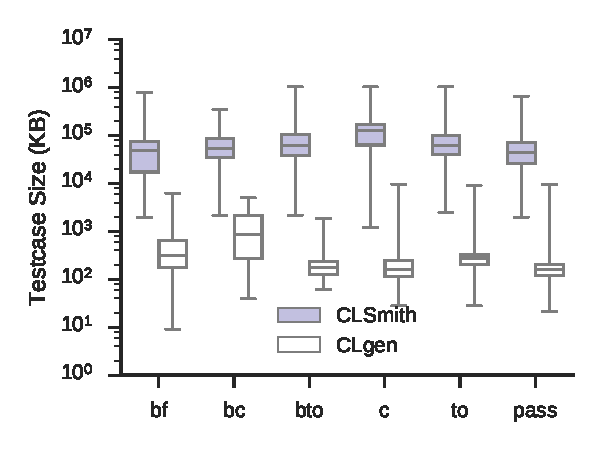
\includegraphics[width=\columnwidth]{build/img/kernel-sizes}%
	\caption{%
		Kernel line counts, grouped by outcome. DeepSmith test-cases are on average two orders of magnitude smaller than CLSmith.%
	}%
	\label{fig:kernel-sizes} %
\end{figure}

\paragraph{Test-case Size}
%SELECT MIN(linecount) as minlen,
%->    AVG(linecount) as meanlen,
%->        MAX(linecount) as maxlen
%-> FROM CLSmithResults results
%-> LEFT JOIN CLSmithMetas meta ON results.id = meta.id
%-> LEFT JOIN CLSmithTestCases testcases ON results.testcase_id = testcases.id
%-> LEFT JOIN CLSmithPrograms programs ON testcases.program_id = programs.id
%-> WHERE cumtime < 48 * 3600;
%+--------+-----------+--------+
%| minlen | meanlen   | maxlen |
%+--------+-----------+--------+
%|     56 | 1186.8496 |  11222 |
%+--------+-----------+--------+
The average CLSmith program is 1189 lines long (excluding headers). CLSmith kernels are unreadable, requiring automatic or manual test-case reduction.
%SELECT MIN(linecount) as minlen,
%->    AVG(linecount) as meanlen,
%->        MAX(linecount) as maxlen
%-> FROM CLgenResults results
%-> LEFT JOIN CLgenMetas meta ON results.id = meta.id
%-> LEFT JOIN CLgenTestCases testcases ON results.testcase_id = testcases.id
%-> LEFT JOIN CLgenPrograms programs ON testcases.program_id = programs.id
%-> WHERE cumtime < 48 * 3600;
%+--------+---------+--------+
%| minlen | meanlen | maxlen |
%+--------+---------+--------+
%|      1 | 20.3163 |    636 |
%+--------+---------+--------+
Average CLgen kernel is 20 lines long.
% SELECT SUM(linecount)
% FROM CLSmithResults results
% INNER JOIN CLSmithMetas meta ON results.id = meta.id
% INNER JOIN CLSmithTestCases testcases ON results.testcase_id = testcases.id
% INNER JOIN CLSmithPrograms programs on testcases.program_id = programs.id
% WHERE cumtime < 48 * 3600;
Over the course of testing, a combined $3.39 \times 10^8$ of CLSmith code was evaluated, compared to $3.76 \times 10^6$ lines of DeepSmith code.

\paragraph{Test-case Reduction} We used a modified version of C-Reduce which supports OpenCL~\cite{Pflanzer2016} to perform automatic test-case, using the default settings. The available implementation supports reduction only of anomalous-output test-cases, though this could be extended to support other outcomes (we did not do this). Test-case reduction is a time-consuming process, even with the parallelized implementation. Figure~\ref{fig:kernel-sizes} shows the runtimes of reductions, and Figure~\cc{TODO} shows the test-case sizes before and after reduction. For CLSmith-generated kernels, test case reduction is necessary to expose the problematic code from within the hundreds of lines of generated program. DeepSmith kernels are on average an order of magnitude smaller. We found that reduction \ldots

% Average GitHub charchounts: 1451
% Average GitHub linecounts: 53

\newsavebox{\IntelPtrAssertion}
\begin{lrbox}{\IntelPtrAssertion}
  \hspace{1.5em}
  \begin{lstlisting}
    __kernel void A(__global int* a, __global int* b) {
      int c = (int)get_global_id(0);
      a[c] += b;
    }
  \end{lstlisting}
\end{lrbox}

\newsavebox{\IntelScalarAssertion}
\begin{lrbox}{\IntelScalarAssertion}
  \hspace{1.5em}
  \begin{lstlisting}
    __kernel void A(__global float* a, __global float* b, __global float* c, __local float* d, unsigned int e, unsigned int f) {
      for (unsigned int g = get_local_id(0) + get_local_size(0); g < get_local_size(0); g += get_local_size(0)) {
        a[2 * get_local_id(0) + 1] = get_local_id(0);
      }
    }
  \end{lstlisting}
\end{lrbox}

\begin{figure}
  \centering %
  \subfloat[Testbeds $3\pm$ assertion during code generation for pointer assignment.]{%
    \noindent\mbox{\parbox{\columnwidth}{\usebox{\IntelPtrAssertion}}}%
    \label{lst:intel-ptr-assertion}
  }\\%
  \subfloat[Testbeds $3\pm$ assertion in scalar type code generation.]{%
    \noindent\mbox{\parbox{\columnwidth}{\usebox{\IntelScalarAssertion}}}%
    \label{lst:intel-scalar-assertion}
  }\\%
  \caption{Kernels which trigger compiler assertions which both CLSmith and DeepSmith exposed.}%
  \label{lst:clsmith-compiler-assertions}%
\end{figure}

In 48 hours of testing, DeepSmith triggered 9 distinct compiler assertions, CLSmith 2. Both of the assertions triggered by CLSmith were also triggered by CLgen.
% Test-case sizes:
%
% SELECT assertion, AVG(linecount)
% FROM CLSmithResults results
% LEFT JOIN CLSmithTestCases testcases ON results.testcase_id = testcases.id
% LEFT JOIN CLSmithPrograms programs ON testcases.program_id = programs.id
% INNER JOIN CLSmithAssertions assertions ON results.stderr_id = assertions.id
% GROUP BY assertion;
%
% CLSmith:
% 'ASSERTION FAILED: (isa<AllocaInst>(ptr) || ptrCandidate.empty()) && \"storing/loading pointers only support private array\"', '1410.8486'
% 'ASSERTION FAILED: iter != pointerOrigMap.end()', '889.0990'
%
% CLgen:
% ASSERTION FAILED: (isa<AllocaInst>(ptr) || ptrCandidate.empty()) && "storing/loading pointers only support private array"	12.5382
% ASSERTION FAILED: 0	86.3295
% ASSERTION FAILED: isScalarType(type)	5.0000
% ASSERTION FAILED: iter != pointerOrigMap.end()	9.5455
% ASSERTION FAILED: Missing parameters for sync instruction	10.0000
% ASSERTION FAILED: Not implemented	7.1579
% ASSERTION FAILED: Not supported	4.7857
% ASSERTION FAILED: sel.hasDoubleType()	4.6364
% ASSERTION FAILED: srcType != ir::TYPE_U64	3.0000
The CLSmith kernels which triggered the two assertions were on average 1411 and 889 lines respectively (excluding headers). The same assertions were triggered with DeepSmith kernels of average 13 lines and 10 lines, respectively. \cc{TODO: listings}
%
% SELECT num, src, assertion
%FROM CLgenResults results
%LEFT JOIN CLgenTestCases testcases ON results.testcase_id = testcases.id
%LEFT JOIN CLgenPrograms programs ON testcases.program_id = programs.id
%LEFT JOIN Configurations ON results.testbed_id = Configurations.id
%INNER JOIN CLgenAssertions assertions ON results.stderr_id = assertions.id
%WHERE assertion = 'ASSERTION FAILED: srcType != ir::TYPE_U64';
We were able to trigger the assertion \emph{srcType != ir::TYPE\_U64} in Testbeds $3\pm$ with only a 3 line test-case.
%
DeepSmith also triggered \emph{unreachable!} compiler errors in 180 distinct test cases, CLSmith triggered 0.

\cc{What is the bug rate per line of code?}


\paragraph{Bug Diversity}

Hard to quantify, but our results suggest the value of our syntactic approach.

% How many GitHub kernels contain 'struct's?
% $ ls | xargs grep -l struct -- | wc -l
% 331
CLSmith is biased towards identifying struct miscompilations, though only 7.1\% of OpenCL kernels on GitHub use them.

Our approach is biased towards identifying bugs in compiler front-ends, since not all generated programms are well formed/well typed. Results suggest we cover more areas of the compiler, E.g. compiler crashes, compiler timeouts, etc.

Oclgrind was resilient to CLSmith testing, yet we managed to trip it up during compilation, and discovered the switch race condition.

Overall, CLSmith is better at finding miscompilations. We believe our approach to be complimentary.

%\begin{figure}
%	\centering %
%	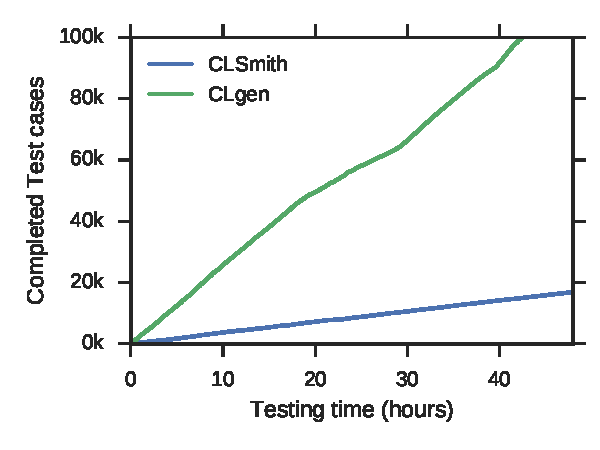
\includegraphics[width=\columnwidth]{build/img/total-tests}%
%	\caption{%
%		Test-cases. \cc{TODO: Replot with the fastest and slowest device for each}%
%	}%
%	\label{fig:total-tests} %
%\end{figure}
